\section{(Alternate) Searching the ELM database using the REST API}
\label{sec:search_REST}

Many researchers are interested in large-scale analyses rather than
information about individual protein sequences. To this end, individual
queries to the ELM webserver with a single protein id at a time, are not
practical.

For this reason, as much information as possible is made available via a
REST interface \cite{Fielding2002}. This allows the user to interact
with the ELM database and ELM webserver via scriptable URL requests.
Each request can easily be tested in the browser before it is being
automated in a script.

In this section we will explore the various ways in which data can
downloaded both in using the browser as well as via the commandline.

%
% Subsection: Necessary Resources
%
\subsection{Necessary Resources}

\subsubsection{Software}

Ideally use \code{curl} https://curl.haxx.se/ on the commandline. This
program can be launched from the terminal in any of the major operating
systems: OSX, Windows and Linux. Of course \code{curl} is only one of
many different ways to access web content programatically, and we
suggest anyone to use which ever program they feel is better suited for
their tasks.

\begin{enumerate}

%
% Subsection: Necessary Resources
%
\subsection{Downloading all ELM
classes}\label{downloading-all-elm-classes}

\begin{figure}[h!]
	\centering
	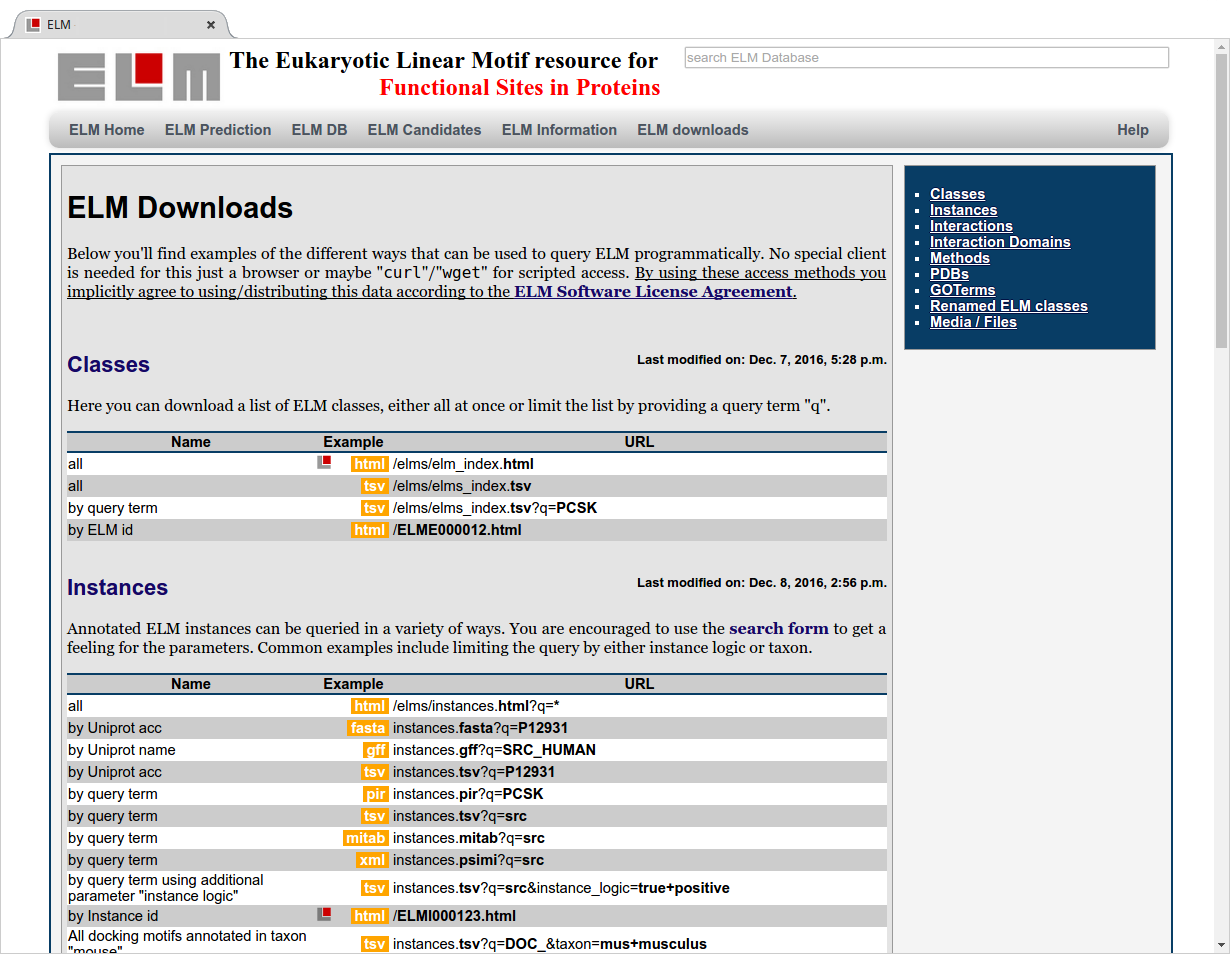
\includegraphics[width=\textwidth]{Figures/search_REST/elm_downloads_html.png}
	\caption{
	The ELM downloads page, which holds
	information about the different types of data (such as ``Classes'',
	``Instances'', etc; see menu to the right) that can be obtained from the
	server. The orange boxes are clickable links, the URL following them are
	used to highlight the URL scheme used by the server (bold font denotes
	specifics used in the examples such as query terms, or formats).
	}
	\label{fig:search_REST_downloads}
\end{figure}

\item Direct your browser to the URL \rurl{elm.eu.org/downloads} or select
	`ELM Downloads' from the main menu
	(Fig. \ref{fig:search_REST_downloads}).
	This page contains links and descriptions on how to download ELM data
	in text format. The datasets are split into several smaller collections
	(for example ``Classes'', ``Instances'', etc). Each table contains
	links (in orange) to download the data in various formats.

	\sdesc{Each table also shows the `last modified date' indicating when
		the data was last updated. This is useful if you want to know
		when to update your local data with the most up to date ELM
		data. }

\item Click on the first orange `html' link in the table ``Classes'' to
	navigate to the following URL:
	\rurl{elm.eu.org/elms/elm\_index.html}. This page shows all of the
	annotated ELM classes in the database. This page is the same one as
	shown in figure \ref{fig:explore_content_elms}.

\item Navidate to the folling URL: \rurl{elm.eu.org/elms.html?q=CSK'}
	specifying \code{q=CSK} to limit the list of ELMs to those matching the
	search query ``CSK''. This page is again similar to the one shown in
	figure \ref{fig:explore_content_elms}, but with less classes.

	\sdesc{ This search result is identical to the result you would obtain
		by doing a ``manual'' search on the ELM Classes page
		described in step 3 of \ref{sec:explore_content}
		(Fig. \ref{fig:explore_content_elms}).}


\item Open the following URL: \rurl{elm.eu.org/elms.tsv?q=CSK} to download a
	list of classes that match the search query ``CSK'' (as in the previous
	step) in the ``tab separated values'' format. By exchanging the
	\fileformat{.html} part of the url with \fileformat{.tsv}', we ask the
	webserver to give us the data in ``tab-separated values'' format.

	\sdesc{ Depending on which browser you are using, the file may open
		directly in your browser, or you may be prompted to download
		the file or save it to a separate location. In the latter two
		cases you can open the downloaded file using a (plain) text
		file viewer, or possible a spreadsheet viewer (such as
		Microsoft Excel or LibreOffice Calc).}

\begin{figure}[h!]
	\centering
	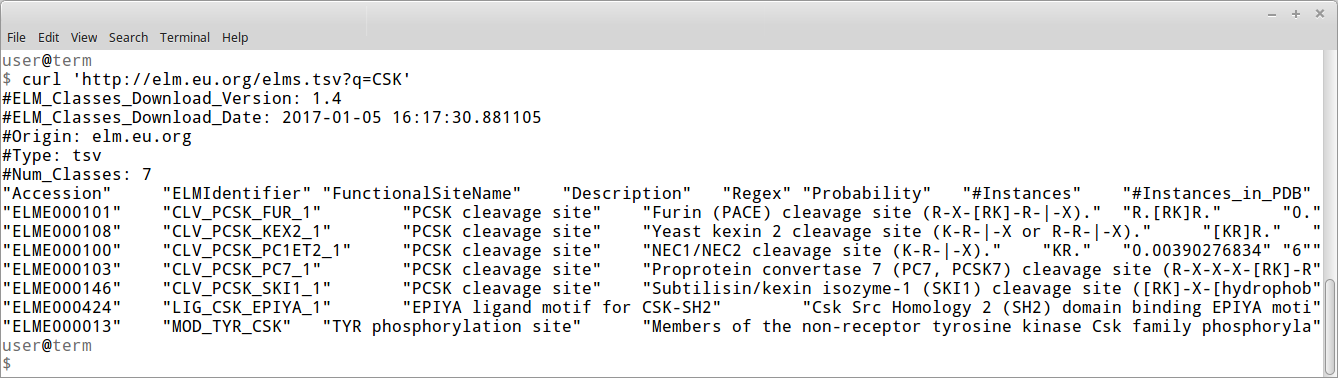
\includegraphics[width=\textwidth]{Figures/search_REST/elm_curl_classes_CSK.png}
	\caption{
	A screenshot of a terminal window using
	\code{curl} to download all ELM classes matching the term `CSK'.
	}
	\label{fig:search_REST_curl_csk}
\end{figure}

\item Type the follwing command into a command line terminal to
	download the same data from the previous step directly into the
	terminal:
	\code{curl 'http://elm.eu.org/elms/elms\_index.tsv?q=CSK'}.  The output
	should look similar to figure \ref{fig:search_REST_curl_csk}.
	The column names are the same ones as shown in the
	table in figure \ref{fig:explore_content_elms}.

	\sdesc{ Use the curl option \code{-o} to save the results directly to
		a file.  For example: \code{curl -o classes.tsv
		'http://elm.eu.org/elms/elms\_index.tsv?q=CSK'} will save the
		data to a file called \emph{classes.tsv}.}

\begin{figure}[h!]
	\centering
	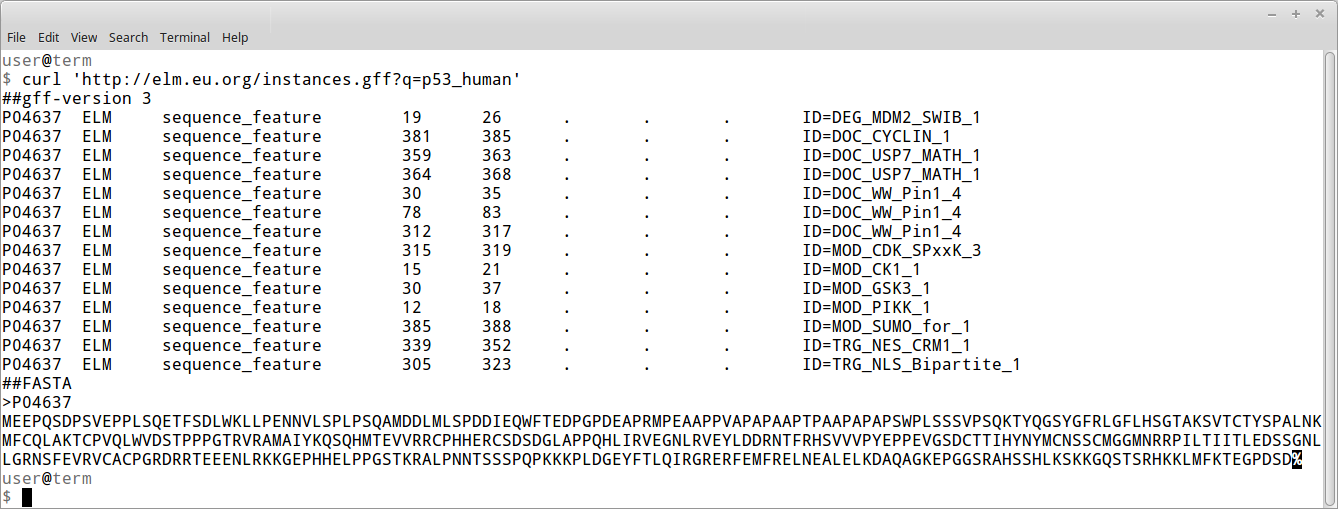
\includegraphics[width=\textwidth]{Figures/search_REST/elm_curl_instances_p53_human.png}
	\caption{
	Screenshot of a terminal window using \code{curl} to download all ELM
	instances annotated for sequence p53\_human.
	}
	\label{fig:search_REST_curl_p53}
\end{figure}

\item To download a list of all motif instances detected in Human P53, type the
	followin command into a terminal: \code{curl
	'http://elm.eu.org/instances.gff?q=p53\_human'}. The output should look
	similar to that shown in figure \ref{fig:predicting_REST_curl_p53}. The
	output is in the ``General Feature Format''
	(see \rurl{www.ensembl.org/info/website/upload/gff.html\#moreinfo}),
	with the FASTA formatted sequence appended to the end of the output.  

	\sdesc{ Many other file formats are available for downloading instances
		annotations, including the \fileformat{fasta},
		\fileformat{gff}, \fileformat{pir}, OR PSI-MI format (either
		\fileformat{xml} or \fileformat{MiTab})}


\item To download a list of all instances matchin th search query ``CLV'' in
	the yellow fever mosquito (\textit{Aedes agypti}), enter the following
	command into a terminal:
	\code{curl `http://elm.eu.org/instances.tsv?q=CLV\&taxon=aedes+aegypti'}.
	In general any species name can be used, always replacing the ``space''
	with a ``+''. This should return a single instance, the only one
	matching CLV in \textit{A. aegypti}.

\item More data (interactions, domains, methods, etc.) can be downloaded from
	ELM in analogous fashion as shown in the preceeding steps. Take a look
	at the ELM Downloads page (http://elm.eu.org/downloads, figure
	\ref{fig:search_REST_downloads}) for an overview of which datasets can
	be downloaded, and what the different possible filters and formats are
	for each dataset.  

\end{enumerate}
